\section{Kernel frameworks for device drivers}

\begin{frame}
  \frametitle{Kernel and Device Drivers}
  \begin{columns}
    \column{0.7\textwidth} In Linux, a driver is always interfacing
    with:
    \begin{itemize}
    \item a {\bf framework} that allows the driver to expose the
      hardware features to user space applications.
    \item a {\bf bus infrastructure}, part of the device model, to
      detect/communicate with the hardware.
    \end{itemize}
    This section focuses on the {\em kernel frameworks}, while the
    {\em bus infrastructure} was covered earlier in this training.
    \column{0.3\textwidth}
    \includegraphics[height=0.8\textheight]{slides/kernel-frameworks/driver-architecture.pdf}
  \end{columns}
\end{frame}

\subsection{User space vision of devices}

\begin{frame}
  \frametitle{Types of devices} Under Linux, there are essentially
  three types of devices:
  \begin{itemize}
  \item {\bf Network devices}. They are represented as network
    interfaces, visible in user space using \code{ip a}
  \item {\bf Block devices}. They are used to provide user space
    applications access to raw storage devices (hard disks, USB
    keys). They are visible to the applications as {\em device files}
    in \code{/dev}.
  \item {\bf Character devices}. They are used to provide user space
    applications access to all other types of devices (input, sound,
    graphics, serial, etc.). They are also visible to the applications
    as {\em device files} in \code{/dev}.
  \end{itemize}
  $\rightarrow$ Most devices are {\em character devices}, so we will
  study these in more details.
\end{frame}

%\begin{frame}
%  \frametitle{Types of devices}
%  \begin{center}
%    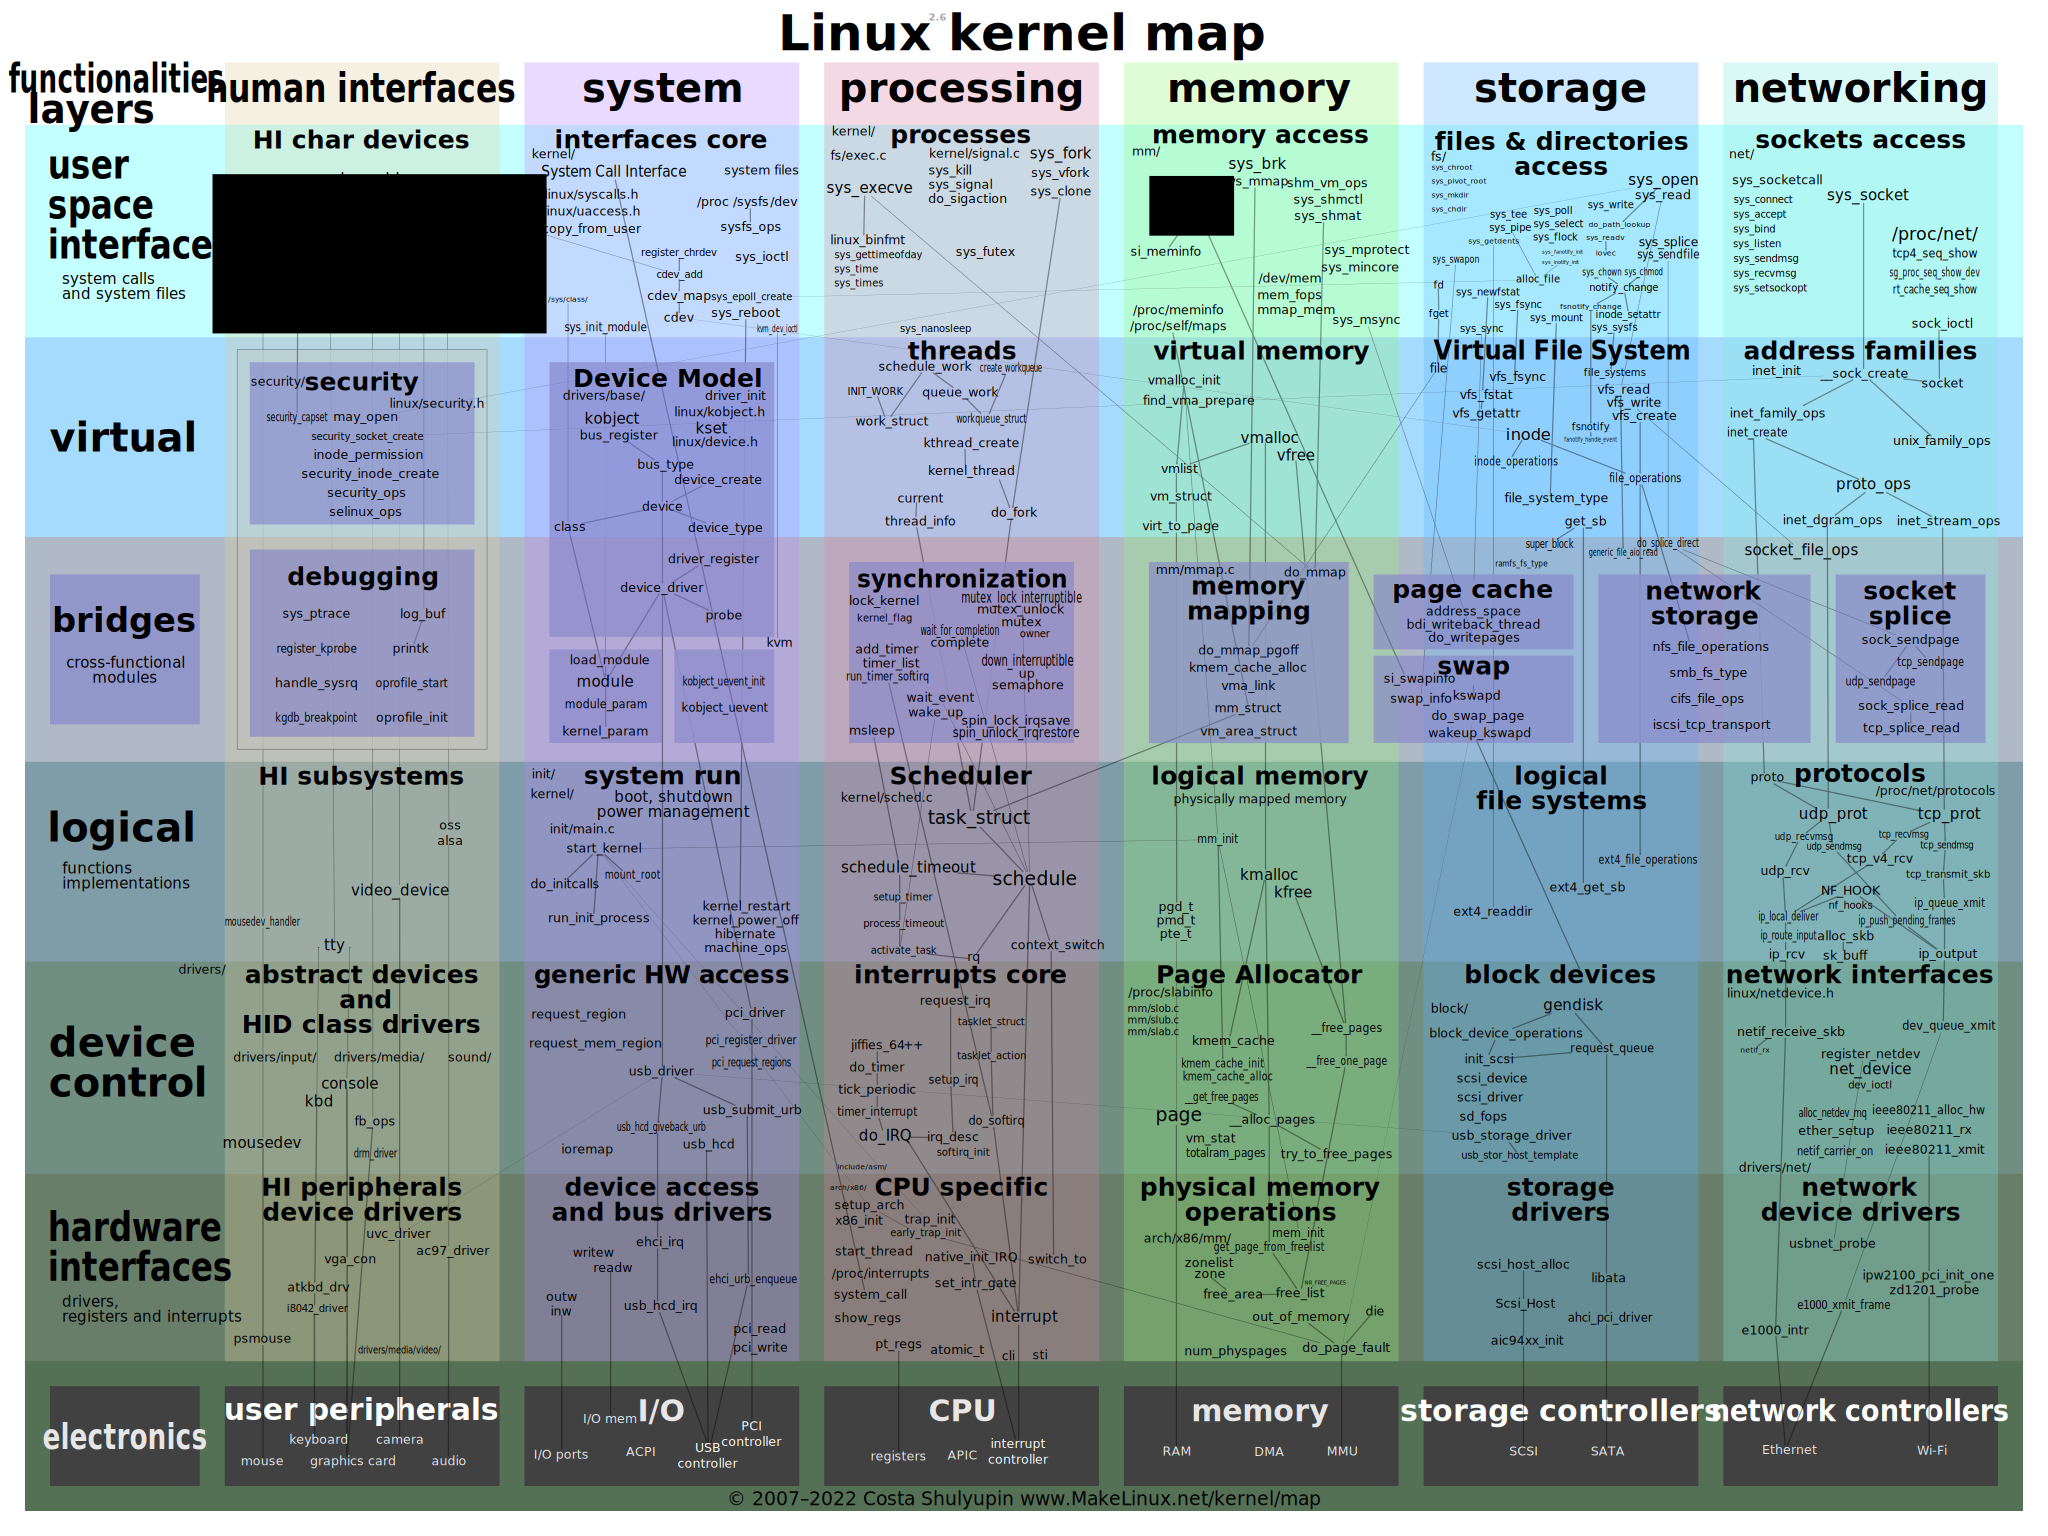
\includegraphics[height=0.9\textheight]{slides/kernel-frameworks/linux_kernel_map.pdf}
%  \end{center}
%\end{frame}

\begin{frame}
  \frametitle{Major and minor numbers}
  \begin{itemize}
  \item Within the kernel, all block and character devices are
    identified using a {\em major} and a {\em minor} number.
  \item The {\em major number} typically indicates the family of the
    device.
  \item The {\em minor number} allows drivers to distinguish
    the various devices they manage.
  \item Most major and minor numbers are statically allocated, and
    identical across all Linux systems.
  \item They are defined in \kdochtml{admin-guide/devices}.
  \end{itemize}
\end{frame}

\begin{frame}
  \frametitle{Devices: everything is a file}
  \begin{itemize}
  \item A very important UNIX design decision was to represent most
    {\em system objects} as files
  \item It allows applications to manipulate all {\em system objects} with
    the normal file API (\code{open}, \code{read}, \code{write},
    \code{close}, etc.)
  \item So, devices had to be represented as files to the applications
  \item This is done through a special artifact called a {\bf device
      file}
  \item It is a special type of file, that associates a file name
    visible to user space applications to the triplet {\em (type,
      major, minor)} that the kernel understands
  \item All {\em device files} are by convention stored in the
    \code{/dev} directory
  \end{itemize}
\end{frame}

\begin{frame}[fragile]
\frametitle{Device files examples}

Example of device files in a Linux system

\small
\begin{verbatim}
$ ls -l /dev/ttyS0 /dev/tty1 /dev/sda /dev/sda1 /dev/sda2 /dev/sdc1 /dev/zero
brw-rw---- 1 root disk    8,  0 2011-05-27 08:56 /dev/sda
brw-rw---- 1 root disk    8,  1 2011-05-27 08:56 /dev/sda1
brw-rw---- 1 root disk    8,  2 2011-05-27 08:56 /dev/sda2
brw-rw---- 1 root disk    8, 32 2011-05-27 08:56 /dev/sdc
crw------- 1 root root    4,  1 2011-05-27 08:57 /dev/tty1
crw-rw---- 1 root dialout 4, 64 2011-05-27 08:56 /dev/ttyS0
crw-rw-rw- 1 root root    1,  5 2011-05-27 08:56 /dev/zero
\end{verbatim}
\normalsize

Example C code that uses the usual file API to write data to a serial port

\small
\begin{minted}{c}
int fd;
fd = open("/dev/ttyS0", O_RDWR);
write(fd, "Hello", 5);
close(fd);
\end{minted}
\end{frame}

\begin{frame}
  \frametitle{Creating device files}
  \begin{itemize}
    \item Before Linux 2.6.32, on basic Linux systems,
    the device files had to be created manually using the
    \code{mknod} command
    \begin{itemize}
    \item \code{mknod /dev/<device> [c|b] major minor}
    \item Needed root privileges
    \item Coherency between device files and devices handled by the
      kernel was left to the system developer
    \end{itemize}
  \item The \code{devtmpfs} virtual filesystem can be mounted on
    \code{/dev} and contains all the devices registered to kernel frameworks.
    The \kconfig{CONFIG_DEVTMPFS_MOUNT} kernel configuration option
    makes the kernel mount it automatically at boot time, except
    when booting on an initramfs.
  \item \code{devtmpfs} can be supplemented by userspace tools like
    \code{udev} or \code{mdev} to adjust permission/ownership, load
    kernel modules automatically and create symbolic links to devices.
  \end{itemize}
\end{frame}

\subsection{Character drivers}

\begin{frame}
  \frametitle{A character driver in the kernel}
  \begin{itemize}
  \item From the point of view of an application, a {\em character
      device} is essentially a {\bf file}.
  \item The driver of a character device must therefore implement {\bf
      operations} that let applications think the device is a file:
    \code{open}, \code{close}, \code{read}, \code{write}, etc.
  \item In order to achieve this, a character driver must implement
    the operations described in the \kstruct{file_operations}
    structure and register them.
  \item The Linux filesystem layer will ensure that the driver's
    operations are called when a user space application makes the
    corresponding system call.
  \end{itemize}
\end{frame}

\begin{frame}
  \frametitle{From user space to the kernel: character devices}
  \begin{center}
    \includegraphics[height=0.8\textheight]{slides/kernel-frameworks/user-kernel-exchanges.pdf}
  \end{center}
\end{frame}

\begin{frame}[fragile]
  \frametitle{File operations}
  Here are the most important operations for a character
  driver, from the definition of \kstruct{file_operations}:
\begin{minted}[fontsize=\footnotesize]{c}
struct file_operations {
    struct module *owner;
    ssize_t (*read) (struct file *, char __user *,
        size_t, loff_t *);
    ssize_t (*write) (struct file *, const char __user *,
        size_t, loff_t *);
    long (*unlocked_ioctl) (struct file *, unsigned int,
        unsigned long);
    int (*mmap) (struct file *, struct vm_area_struct *);
    int (*open) (struct inode *, struct file *);
    int (*release) (struct inode *, struct file *);
    ...
};
\end{minted}
Many more operations exist. All of them are optional.
\end{frame}

\begin{frame}[fragile]
  \frametitle{open() and release()}
  \begin{itemize}
  \item \mint{c}+int foo_open(struct inode *i, struct file *f)+
    \begin{itemize}
    \item Called when user space opens the device file.
    \item {\bf Only implement this function when you do something
          special with the device at \code{open()} time.}
    \item \kstruct{inode} is a structure that uniquely represents a file
      in the filesystem (be it a regular file, a directory, a symbolic
      link, a character or block device)
    \item \kstruct{file} is a structure created every time a file is
      opened. Several file structures can point to the same
      \code{inode} structure.
      \begin{itemize}
      \item Contains information like the current position, the
        opening mode, etc.
      \item Has a \code{void *private_data} pointer that one can
        freely use.
      \item A pointer to the \ksym{file} structure is passed to all other
        operations
      \end{itemize}
    \end{itemize}
  \item \mint{c}+int foo_release(struct inode *i, struct file *f)+
    \begin{itemize}
    \item Called when user space closes the file.
    \item {\bf Only implement this function when you do something
          special with the device at \code{close()} time.}
    \end{itemize}
  \end{itemize}
\end{frame}

\begin{frame}[fragile]
  \frametitle{read() and write()}
  \begin{itemize}
  \item \mint[fontsize=\small]{c}+ssize_t foo_read(struct file *f, char __user *buf, size_t sz, loff_t *off)+
    \begin{itemize}
    \item Called when user space uses the \code{read()} system call on
      the device.
    \item Must read data from the device, write at most \code{sz}
      bytes to the user space buffer \code{buf}, and update the
      current position in the file \code{off}. \code{f} is a pointer
      to the same file structure that was passed in the \code{open()}
      operation
    \item Must return the number of bytes read.\\
	  \code{0} is usually interpreted by userspace as the end of
          the file.
    \item On UNIX, \code{read()} operations typically block when there
      isn't enough data to read from the device
    \end{itemize}
  \item \mint[fontsize=\small]{c}+ssize_t foo_write(struct file *f, const char __user *buf, size_t sz, loff_t *off)+
    \begin{itemize}
    \item Called when user space uses the \code{write()} system call
      on the device
    \item The opposite of \code{read}, must read at most \code{sz}
      bytes from \code{buf}, write it to the device, update \code{off}
      and return the number of bytes written.
    \end{itemize}
  \end{itemize}
\end{frame}

\begin{frame}
  \frametitle{Exchanging data with user space 1/3}
  \begin{itemize}
  \item Kernel code isn't allowed to directly access user space
    memory, using \kfunc{memcpy} or direct pointer dereferencing
    \begin{itemize}
    \item User pointer dereferencing is disabled by default to make it
      harder to exploit vulnerabilities.
    \item If the address passed by the application was invalid, the
      kernel could segfault.
    \item {\bf Never} trust user space. A malicious application could
      pass a kernel address which you could overwrite with device data
      (\code{read} case), or which you could dump to the device
      (\code{write} case).
    \item Doing so does not work on some architectures anyway.
    \end{itemize}
  \item To keep the kernel code portable, secure, and have proper
    error handling, your driver must use special kernel functions
    to exchange data with user space.
  \end{itemize}
\end{frame}

\begin{frame}[fragile]
  \frametitle{Exchanging data with user space 2/3}
  \begin{itemize}
  \item A single value
    \begin{itemize}
    \item \code{get_user(v, p);}
      \begin{itemize}
      \item The kernel variable \code{v} gets the value pointed by the
        user space pointer \code{p}
      \end{itemize}
    \item \code{put_user(v, p);}
      \begin{itemize}
      \item The value pointed by the user space pointer \code{p} is
        set to the contents of the kernel variable \code{v}.
      \end{itemize}
    \end{itemize}
  \item A buffer
    \begin{itemize}
    \item \mint{c}+unsigned long copy_to_user(void __user *to,+
      \mint{c}+const void *from, unsigned long n);+
    \item \mint{c}+unsigned long copy_from_user(void *to,+
      \mint{c}+const void __user *from, unsigned long n);+
    \end{itemize}
  \item The return value must be checked. Zero on success, non-zero on
    failure. If non-zero, the convention is to return \code{-}\ksym{EFAULT}.
  \end{itemize}
\end{frame}

\begin{frame}
 \frametitle{Exchanging data with user space 3/3}
 \begin{center}
    \includegraphics[height=0.8\textheight]{slides/kernel-frameworks/copy-to-from-user.pdf}
 \end{center}
\end{frame}

\begin{frame}
  \frametitle{Zero copy access to user memory}
  \begin{itemize}
  \item Having to copy data to or from an intermediate kernel buffer
    can become expensive when the amount of data to transfer is
    large (video).
  \item \emph{Zero copy} options are possible:
    \begin{itemize}
    \item \code{mmap()} system call to allow user space to directly
      access memory mapped I/O space. See our \code{mmap()} chapter.
    \item \kfunc{get_user_pages} and related functions to get a
      mapping to user pages without having to copy them.
    \end{itemize}
  \end{itemize}
\end{frame}

\begin{frame}[fragile]
  \frametitle{unlocked\_ioctl()}
  \begin{itemize}
  \item \mint[fontsize=\small]{c}+long unlocked_ioctl(struct file *f, unsigned int cmd, unsigned long arg)+
    \begin{itemize}
    \item Associated to the \code{ioctl()} system call.
    \item Called unlocked because it didn't hold the Big Kernel Lock
      (gone now).
    \item Allows to extend the driver capabilities beyond the limited
      read/write API.
    \item For example: changing the speed of a serial port, setting
      video output format, querying a device serial number... Used
      extensively in the V4L2 (video) and ALSA (sound) driver frameworks.
    \item \code{cmd} is a number identifying the operation to perform.\\
      See \kdochtml{driver-api/ioctl} for the recommended way of choosing
      \code{cmd} numbers.
    \item \code{arg} is the optional argument passed as third argument
      of the \code{ioctl()} system call. Can be an integer, an
      address, etc.
    \item The semantic of \code{cmd} and \code{arg} is
      driver-specific.
    \end{itemize}
  \end{itemize}
\end{frame}

\begin{frame}[fragile]
  \frametitle{ioctl() example: kernel side}
\begin{minted}[fontsize=\tiny]{c}
#include <linux/phantom.h>

static long phantom_ioctl(struct file *file, unsigned int cmd,
    unsigned long arg)
{
    struct phm_reg r;
    void __user *argp = (void __user *)arg;

    switch (cmd) {
    case PHN_SET_REG:
        if (copy_from_user(&r, argp, sizeof(r)))
            return -EFAULT;
        /* Do something */
        break;
    ...
    case PHN_GET_REG:
        if (copy_to_user(argp, &r, sizeof(r)))
            return -EFAULT;
        /* Do something */
        break;
    ...
    default:
        return -ENOTTY;
    }

    return 0;
}
\end{minted}
\small Selected excerpt from \kfile{drivers/misc/phantom.c}
\end{frame}

\begin{frame}[fragile]
  \frametitle{ioctl() Example: Application Side}
\begin{minted}[fontsize=\footnotesize]{c}
#include <linux/phantom.h>

int main(void)
{
    int fd, ret;
    struct phm_reg reg;

    fd = open("/dev/phantom");
    assert(fd > 0);

    reg.field1 = 42;
    reg.field2 = 67;

    ret = ioctl(fd, PHN_SET_REG, &reg);
    assert(ret == 0);

    return 0;
}
\end{minted}
\end{frame}

\begin{frame}
  \frametitle{Allocating a major / minor number}
  Before registering a character device, it is necessary to obtain a
  major and minor number:
  \begin{itemize}
    \item A major / minor number is stored in an opaque type \ksym{dev_t} (currently a \ksym{u32}).
          It should not be accessed directly! Instead:
    \begin{itemize}
      \item Create a \ksym{dev_t} using \kfunc{MKDEV}.
      \item Retrieve the major / minor number with \kfunc{MAJOR} and \kfunc{MINOR}.
    \end{itemize}
    \item Some major / minor numbers are statically allocated.
          In this case, \kfunc{register_chrdev_region} is used.
          %See the list of registered numbers in \kfile{Documentation/admin-guide/devices.txt}.
          See the list of registered numbers in \kdochtml{admin-guide/devices}.
    \item It is recommended to allocate a \ksym{dev_t} dynamically instead:
    \begin{itemize}
      \item Allocate one (or several) number(s) using \kfunc{alloc_chrdev_region}.
      \item Release it using \kfunc{unregister_chrdev_region}.
    \end{itemize}
  \end{itemize}
\end{frame}

\begin{frame}
  \frametitle{Registering a character device}
  The registration of a character device is done using a \kstruct{cdev}:
  \begin{itemize}
    \item Either it can be dynamically allocated with \kfunc{cdev_alloc}.
    \item Or, if the structure is static, it should be initialized using \kfunc{cdev_init}.
    \item In both cases, a pointer to the \kstruct{file_operations} is stored inside \kstruct{cdev}.
  \end{itemize}

  Finally the registration is performed using \kfunc{cdev_add}.
  When the character device is no longer needed, use \kfunc{cdev_del} to delete it.
\end{frame}

% other examples:
%   drivers/char/mem.c
%   drivers/char/scx200_gpio.c
%   drivers/misc/phantom.c
\begin{frame}[fragile]
  \frametitle{Registering a character device: example}
\begin{minted}[fontsize=\footnotesize]{c}
static dev_t first;

static int __init dax_attach(void)
{
    ...
    if (alloc_chrdev_region(&first, 0, 1, DAX_NAME) < 0) {
        dax_err("alloc_chrdev_region failed");
        ret = -ENXIO;
        goto done;
    }
    cdev_init(&c_dev, &dax_fops);
    if (cdev_add(&c_dev, first, 1) == -1) {
        dax_err("cdev_add failed");
        ret = -ENXIO;
        goto cdev_error;
    }
    ...
}
\end{minted}
  \small Selected excerpt from \kfile{drivers/sbus/char/oradax.c}
\end{frame}

\subsection{The concept of kernel frameworks}

\begin{frame}
  \frametitle{Beyond character drivers: kernel frameworks}
  \begin{itemize}
  \item Many device drivers are not implemented directly as character
    drivers
  \item They are implemented under a \emph{framework}, specific to a
    given device type (framebuffer, V4L, serial, etc.)
    \begin{itemize}
    \item The framework allows to factorize the common parts of
      drivers for the same type of devices
    \item From user space, they are still seen as character devices by
      the applications
    \item The framework allows to provide a coherent user space
      interface (\code{ioctl}, etc.) for every type of device,
      regardless of the driver
    \end{itemize}
  \end{itemize}
\end{frame}

\begin{frame}
  \frametitle{Example: Some Kernel Frameworks}
  \begin{center}
    \includegraphics[height=0.8\textheight]{slides/kernel-frameworks/frameworks.pdf}
  \end{center}
\end{frame}

\begin{frame}
  \frametitle{Example: Framebuffer Framework}
  \begin{itemize}
  \item Kernel option \kconfig{CONFIG_FB}
    \begin{itemize}
    \item \code{menuconfig FB}
      \begin{itemize}
      \item \code{tristate "Support for frame buffer devices"}
      \end{itemize}
    \end{itemize}
  \item Implemented in C files in \kdir{drivers/video/fbdev/core}
  \item Defines the user/kernel API
    \begin{itemize}
    \item \kfile{include/uapi/linux/fb.h} (constants and structures)
    \end{itemize}
  \item Defines the set of operations a framebuffer driver must
    implement and helper functions for the drivers
    \begin{itemize}
    \item \kstruct{fb_ops}
    \item \kfile{include/linux/fb.h}
    \end{itemize}
  \end{itemize}
\end{frame}

\begin{frame}[fragile]
  \frametitle{Framebuffer driver operations}
  \small Here are the operations a framebuffer driver can or must
  implement, and define them in a \kstruct{fb_ops} structure
  (excerpt from \kfile{drivers/video/fbdev/skeletonfb.c})
  \footnotesize
  \begin{minted}[fontsize=\scriptsize]{c}
static struct fb_ops xxxfb_ops = {
    .owner = THIS_MODULE,
    .fb_open = xxxfb_open,
    .fb_read = xxxfb_read,
    .fb_write = xxxfb_write,
    .fb_release = xxxfb_release,
    .fb_check_var = xxxfb_check_var,
    .fb_set_par = xxxfb_set_par,
    .fb_setcolreg = xxxfb_setcolreg,
    .fb_blank = xxxfb_blank,
    .fb_pan_display = xxxfb_pan_display,
    .fb_fillrect = xxxfb_fillrect,             /* Needed !!! */
    .fb_copyarea = xxxfb_copyarea,             /* Needed !!! */
    .fb_imageblit = xxxfb_imageblit,           /* Needed !!! */
    .fb_cursor = xxxfb_cursor,                 /* Optional !!! */
    .fb_rotate = xxxfb_rotate,
    .fb_sync = xxxfb_sync,
    .fb_ioctl = xxxfb_ioctl,
    .fb_mmap = xxxfb_mmap,
};
  \end{minted}
\end{frame}

\begin{frame}[fragile]
  \frametitle{Framebuffer driver code}
  \begin{itemize}
  \item In the \code{probe()} function, registration of the
    framebuffer device and operations
  \begin{minted}[fontsize=\footnotesize]{c}
static int xxxfb_probe (struct pci_dev *dev, const struct pci_device_id *ent)
{
    struct fb_info *info;
    [...]
    info = framebuffer_alloc(sizeof(struct xxx_par), device);
    [...]
    info->fbops = &xxxfb_ops;
    [...]
    if (register_framebuffer(info) < 0)
        return -EINVAL;
    [...]
}
  \end{minted}
  \item \kfunc{register_framebuffer} will create a new character device
    in {\em devtmpfs} that can be used by user space applications
    with the generic framebuffer API.
\end{itemize}
\end{frame}

\subsection{The misc subsystem}

\begin{frame}{Why a {\em misc} subsystem?}
  \begin{itemize}
  \item The kernel offers a large number of {\bf frameworks} covering
    a wide range of device types: input, network, video, audio,
    etc.
    \begin{itemize}
    \item These frameworks allow to factorize common functionality
      between drivers and offer a consistent API to user space
      applications.
    \end{itemize}
  \item However, there are some devices that {\bf really do not fit in any
    of the existing frameworks}.
    \begin{itemize}
    \item Highly customized devices implemented in a FPGA, or other
      weird devices for which implementing a complete framework is not
      useful.
    \end{itemize}
  \item The drivers for such devices could be implemented directly as
    raw {\em character drivers} (with \kfunc{cdev_init} and
    \kfunc{cdev_add}).
  \item But there is a subsystem that makes this work a little bit
    easier: the {\bf misc subsystem}.
    \begin{itemize}
    \item It is really only a {\bf thin layer} above the {\em character
        driver} API.
    \item Another advantage is that devices are integrated in the Device
        Model (device files appearing in {\em devtmpfs}, which you don't
	have with raw character devices).
    \end{itemize}
  \end{itemize}
\end{frame}

\begin{frame}{Misc subsystem diagram}
  \begin{center}
    \includegraphics[width=\textwidth]{slides/kernel-frameworks//misc-subsystem-diagram.pdf}
  \end{center}
\end{frame}

\begin{frame}[fragile]{Misc subsystem API (1/2)}
  \begin{itemize}
  \item The misc subsystem API mainly provides two functions, to
    register and unregister {\bf a single} {\em misc device}:
    \begin{itemize}
    \item \code{int misc_register(struct miscdevice * misc);}
    \item \code{void misc_deregister(struct miscdevice *misc);}
    \end{itemize}
  \item A {\em misc device} is described by a \kstruct{miscdevice}
    structure:
    \begin{minted}[fontsize=\footnotesize]{c}
struct miscdevice  {
        int minor;
        const char *name;
        const struct file_operations *fops;
        struct list_head list;
        struct device *parent;
        struct device *this_device;
        const char *nodename;
        umode_t mode;
};
\end{minted}
  \end{itemize}
\end{frame}

\begin{frame}[fragile]{Misc subsystem API (2/2)}
  The main fields to be filled in \kstruct{miscdevice} are:
  \begin{itemize}
  \item \code{minor}, the minor number for the device, or
    \ksym{MISC_DYNAMIC_MINOR} to get a minor number automatically
    assigned.
  \item \code{name}, name of the device, which will be used to create
    the device node if {\em devtmpfs} is used.
  \item \code{fops}, pointer to the same \kstruct{file_operations} structure
    that is used for raw character drivers, describing which functions
    implement the {\em read}, {\em write}, {\em ioctl}, etc. operations.
  \item \code{parent}, pointer to the \code{struct device} of the
    underlying ``physical'' device (platform device, I2C device, etc.)
  \end{itemize}
\end{frame}

\begin{frame}{User space API for misc devices}
  \begin{itemize}
  \item {\em misc devices} are regular character devices
  \item The operations they support in user space depends on the
    operations the kernel driver implements:
    \begin{itemize}
    \item The \code{open()} and \code{close()} system calls to
      open/close the device.
    \item The \code{read()} and \code{write()} system calls to
      read/write to/from the device.
    \item The \code{ioctl()} system call to call some driver-specific
      operations.
    \end{itemize}
  \end{itemize}
\end{frame}

\begin{frame}[fragile]
  \frametitle{Example of a misc device}
\begin{minted}[fontsize=\scriptsize]{c}
static const struct file_operations adi_fops = {
    .read        = adi_read,
    .write       = adi_write,
    ...
};
static struct miscdevice adi_miscdev = {
    .minor = MISC_DYNAMIC_MINOR,
    .name = KBUILD_MODNAME,
    .fops = &adi_fops,
};
static int __init adi_init(void)
{
    return misc_register(&adi_miscdev);
}
static void __exit adi_exit(void)
{
    misc_deregister(&adi_miscdev);
}
module_init(adi_init);
module_exit(adi_exit);
\end{minted}
  \small Selected excerpt from \kfile{drivers/char/adi.c}
\end{frame}

\subsection{Driver data structures and links}

\begin{frame}
  \frametitle{Driver-specific Data Structure}
  \begin{itemize}
  \item Each \emph{framework} defines a structure that a device driver
    must register to be recognized as a device in this framework
    \begin{itemize}
    \item \kstruct{uart_port} for serial ports, \kstruct{net_device} for network
      devices, \kstruct{fb_info} for framebuffers, etc.
    \end{itemize}
  \item In addition to this structure, the driver usually needs to
    store additional information about each device
  \item This is typically done
    \begin{itemize}
    \item By subclassing the appropriate framework structure
    \item By storing a reference to the appropriate framework
      structure
    \item Or by including your information in the framework structure
    \end{itemize}
  \end{itemize}
\end{frame}

\begin{frame}[fragile]
  \frametitle{Driver-specific Data Structure Examples 1/2}
  \begin{itemize}
  \item i.MX serial driver: \kstruct{imx_port} is a subclass of
    \kstruct{uart_port}
  \begin{minted}[fontsize=\scriptsize]{c}
struct imx_port {
    struct uart_port port;
    struct timer_list timer;
    unsigned int old_status;
    int txirq, rxirq, rtsirq;
    unsigned int have_rtscts:1;
    [...]
};
  \end{minted}
  \item ds1305 RTC driver: \kstruct{ds1305} has a reference to
    \kstruct{rtc_device}
  \begin{minted}[fontsize=\scriptsize]{c}
struct ds1305 {
    struct spi_device       *spi;
    struct rtc_device       *rtc;
    [...]
};
  \end{minted}
  \end{itemize}
\end{frame}

\begin{frame}[fragile]
  \frametitle{Driver-specific Data Structure Examples 2/2}
  \begin{itemize}
  \item rtl8150 network driver: \kstruct{rtl8150} has a reference to
    \kstruct{net_device} and is allocated within that framework structure.
  \begin{minted}[fontsize=\scriptsize]{c}
struct rtl8150 {
    unsigned long flags;
    struct usb_device *udev;
    struct tasklet_struct tl;
    struct net_device *netdev;
    [...]
};
  \end{minted}
  \end{itemize}
\end{frame}

\begin{frame}
  \frametitle{Links between structures 1/4}
  \begin{itemize}
  \item The framework structure typically contains a \kstruct{device} \code{*}
    pointer that the driver must point to the corresponding
    \kstruct{device}
    \begin{itemize}
    \item It's the relationship between the logical device (for example a
      network interface) and the physical device (for example the USB
      network adapter)
    \end{itemize}
  \item The device structure also contains a \code{void *} pointer
    that the driver can freely use.
    \begin{itemize}
    \item It's often used to link back the device to the higher-level
      structure from the framework.
    \item It allows, for example, from the \kstruct{platform_device}
      structure, to find the structure describing the logical device
    \end{itemize}
  \end{itemize}
\end{frame}

\begin{frame}[fragile]
  \frametitle{Links between structures 2/4}
  \begin{columns}
    \column{0.7\textwidth}
    \begin{minted}[fontsize=\tiny]{c}
static int serial_imx_probe(struct platform_device *pdev)
{
    struct imx_port *sport; /* per device structure */
    [...]
    sport = devm_kzalloc(&pdev->dev, sizeof(*sport), GFP_KERNEL);
    [...]
    /* setup the link between uart_port and the struct
     * device inside the platform_device */
    sport->port.dev = &pdev->dev;                                // Arrow 1
    [...]
    /* setup the link between the struct device inside
     * the platform device to the imx_port structure */
    platform_set_drvdata(pdev, sport);                           // Arrow 2
    [...]
    uart_add_one_port(&imx_reg, &sport->port);
}

static int serial_imx_remove(struct platform_device *pdev)
{
    /* retrieve the imx_port from the platform_device */
    struct imx_port *sport = platform_get_drvdata(pdev);
    [...]
    uart_remove_one_port(&imx_reg, &sport->port);
    [...]
}
    \end{minted}
    \column{0.3\textwidth}
    \begin{center}
      \includegraphics[height=0.8\textheight]{slides/kernel-frameworks/link-structures-imx.pdf}
    \end{center}
  \end{columns}
\end{frame}

\begin{frame}[fragile]
  \frametitle{Links between structures 3/4}
  \begin{columns}
    \column{0.7\textwidth}
    \begin{minted}[fontsize=\tiny]{c}
static int ds1305_probe(struct spi_device *spi)
{
    struct ds1305                   *ds1305;

    [...]

    /* set up driver data */
    ds1305 = devm_kzalloc(&spi->dev, sizeof(*ds1305), GFP_KERNEL);
    if (!ds1305)
            return -ENOMEM;
    ds1305->spi = spi;                         // Arrow 1
    spi_set_drvdata(spi, ds1305);              // Arrow 2

    [...]

    ds1305->rtc = devm_rtc_allocate_device(&spi->dev); 
                                               // Arrows 3 and 4

    [...]
}

static int ds1305_remove(struct spi_device *spi)
{
    struct ds1305 *ds1305 = spi_get_drvdata(spi);

    [...]
}
    \end{minted}
    \column{0.3\textwidth}
    \begin{center}
      \includegraphics[height=0.8\textheight]{slides/kernel-frameworks/link-structures-rtc.pdf}
    \end{center}
  \end{columns}
\end{frame}

\begin{frame}[fragile]
  \frametitle{Links between structures 4/4}
  \begin{columns}
    \column{0.7\textwidth}
    \begin{minted}[fontsize=\tiny]{c}
static int rtl8150_probe(struct usb_interface *intf,
    const struct usb_device_id *id)
{
    struct usb_device *udev = interface_to_usbdev(intf);
    rtl8150_t *dev;
    struct net_device *netdev;

    netdev = alloc_etherdev(sizeof(rtl8150_t));
    dev = netdev_priv(netdev);

    [...]

    dev->udev = udev;      // Arrow 1
    dev->netdev = netdev;  // Arrow 2

    [...]

    usb_set_intfdata(intf, dev);        // Arrow 3
    SET_NETDEV_DEV(netdev, &intf->dev); // Arrow 4

    [...]
}

static void rtl8150_disconnect(struct usb_interface *intf)
{
    rtl8150_t *dev = usb_get_intfdata(intf);

    [...]
}
    \end{minted}
    \column{0.3\textwidth}
    \begin{center}
      \includegraphics[height=0.8\textheight]{slides/kernel-frameworks/link-structures-netdev.pdf}
    \end{center}
  \end{columns}
\end{frame}
